\chapter{Introduction}\label{1}

This chapter discusses the motivation, specific context, research gaps of literature, goals and research questions, overall methodological approach, and the list of scientific contributions.

\section{Background and Motivation}\label{Background}

To combat climate change, the production of greenhouse gas emissions must be reduced to significant levels and shift to the use of Renewable Energy Sources (\gls{RES}) must be accomplished. In numbers, the European Union's (\gls{EU}) Nationally Determined Contribution (NDC) under the Paris Agreement is to reduce greenhouse gas emissions by at least 40\% by 2030 when compared to 1990 \cite{agreement2015unfccc}. 

The plans involve a future target of nearly 70 GW to 150 GW offshore wind power in the North Sea by 2040. A scope of 140 to 450 GW of offshore wind power in the \gls{EU} by 2050 is seen from the latest European Commission situations. Going with the current pace, the rate of offshore wind energy deployment is deficient in reaching the objectives of the Paris Agreement. To comply with these objectives, an extraordinary jump in offshore wind energy is required, as shown in Figure \ref{fig:Paris_roll_out}. An effective solution calls for an increase in large scale offshore wind energy deployment in the North Sea \cite{noauthor_vision_2020}. As part of the North Sea Wind Power Hub Programme \cite{noauthor_tennet_2020}, the Transmission System Operator (TSO) of the Netherlands, TenneT, has already entered into an innovation partnership with its suppliers to establish a 2 GW offshore platform to bring in their contribution towards the Paris Agreement. Likewise, Denmark is progressing with the first hub-and-spoke energy island with a vision of connecting at least 10 GW of offshore wind power in the North Sea \cite{noauthor_first_2020}. While the requirement for large scale offshore networks is appealing, the technical challenges that could be encountered should also be considered.  

\begin{figure}[H]
\centering
%\hspace*{-1.2cm}
    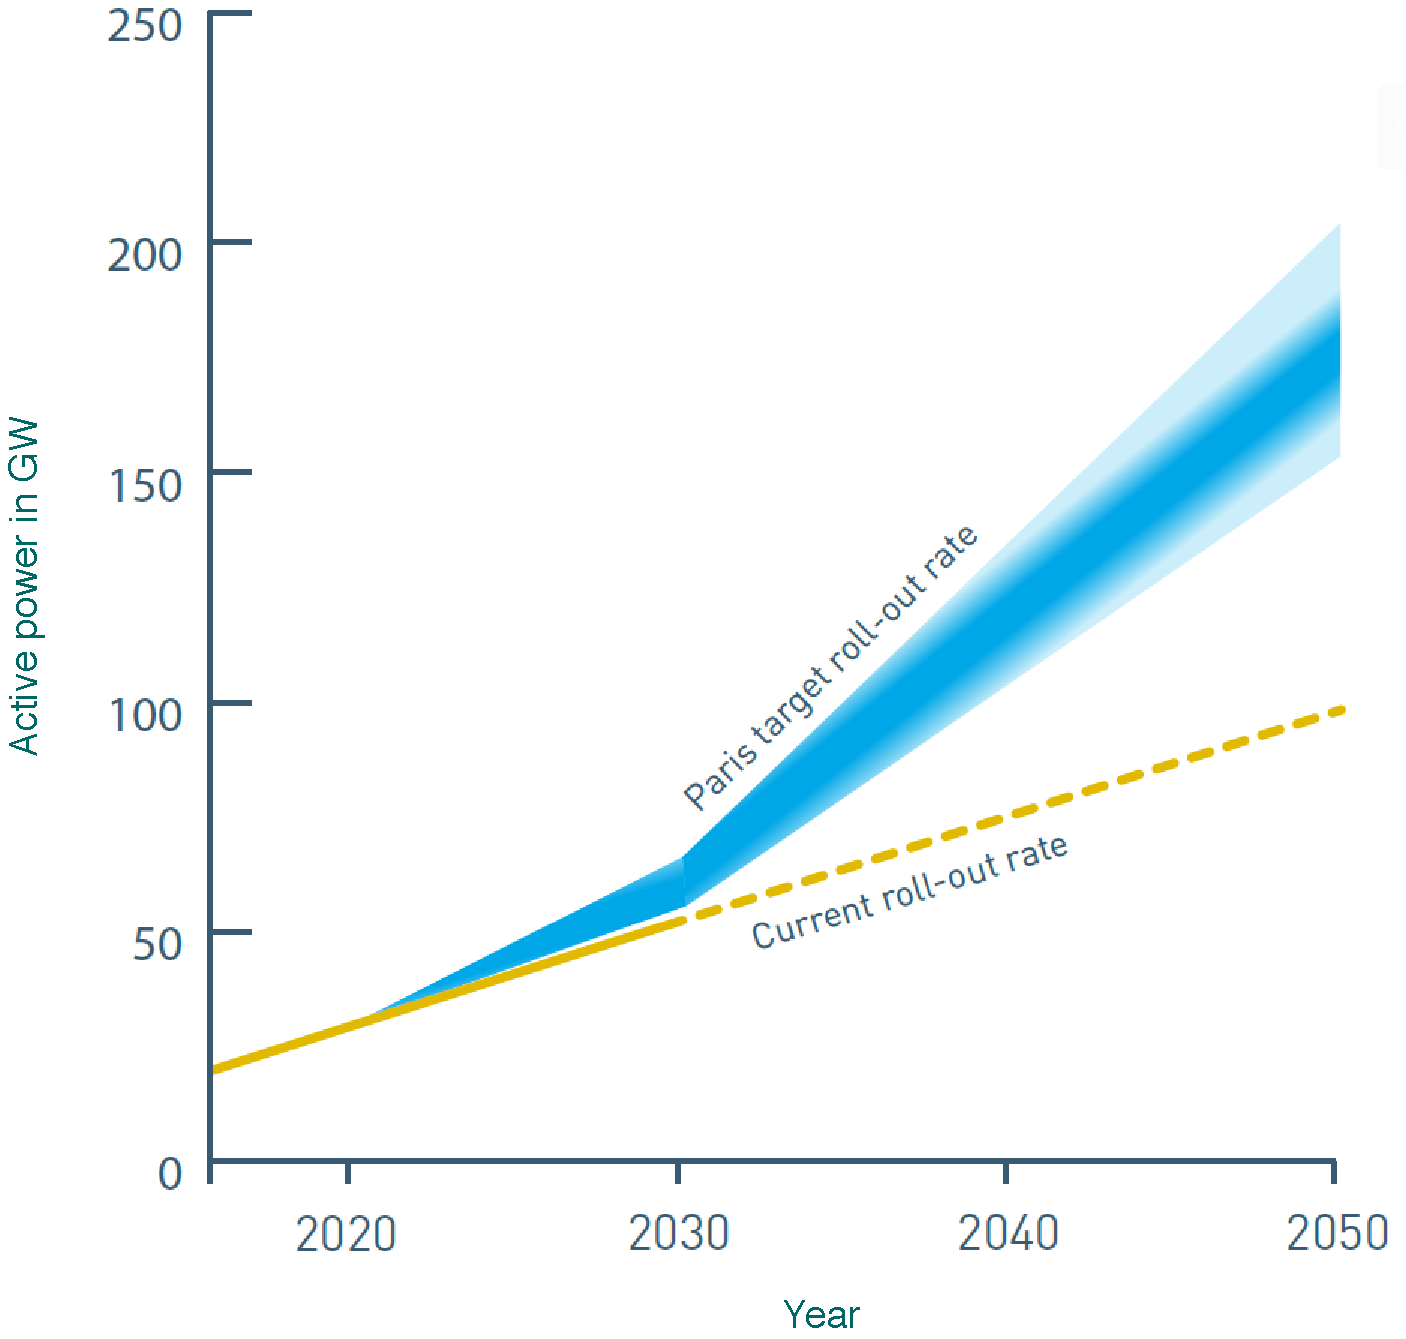
\includegraphics[height = 8.5cm,width = 9cm]{Diagrams/Chapter_1/Paris.pdf}
    \caption{Installed wind capacity in the North Sea in GW \cite{noauthor_vision_2020}}
    \label{fig:Paris_roll_out}
\end{figure}

\gls{RES} are connected to the power system through Power Electronic (\gls{PE}) converters as shown in Figure \ref{fig:Energy_conv_system_2}. The \gls{PE} converters do not possess inherent inertial response characteristics. Until now, integration of \gls{RES} to the power system has not created major problems since the stability of the system is maintained by the synchronous machines in power plants. Traditionally, the inertia for the power system is provided by these synchronous machines connected to the network (Figure \ref{fig:Energy_conv_system}). However, an increase in \gls{RES} in the future causes an increase in \gls{PE} converter based generation units. Simultaneously, the synchronous machines in the conventional power plants need to be disconnected from the network. This makes the power systems weak due to low short circuit power and low system inertia. Therefore, the consequence of disconnecting the synchronous generators leads to the requirement of the \gls{PE} converter based generation units to take up the role of governing the stability of the power system.

\begin{figure}[H]
\centering
%\hspace*{-1.2cm}
    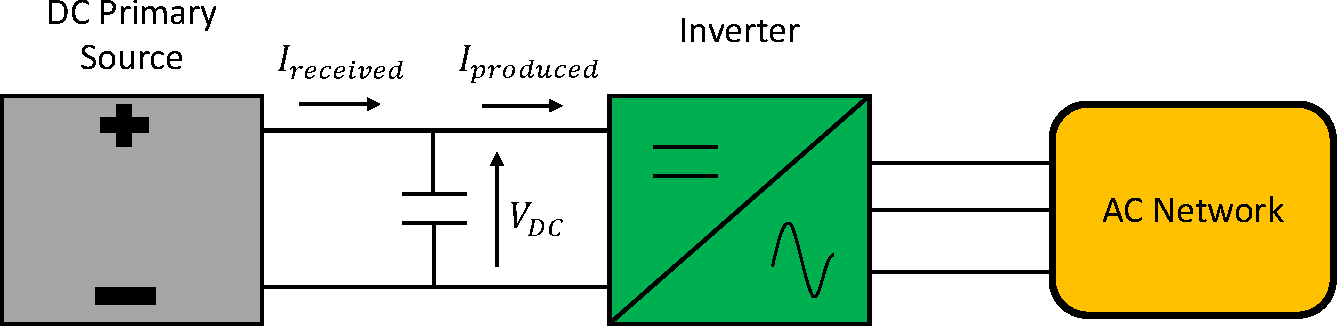
\includegraphics[height = 3cm,width = 12cm]{Diagrams/Chapter_1/Energy_conv_system_2.pdf}
    \caption{PE converter-based generation connection to the AC network \cite{denis_migrate_2018}}
    \label{fig:Energy_conv_system_2}
\end{figure}
\vspace{0mm}
\begin{figure}[H]
\centering
%\hspace*{-1.2cm}
    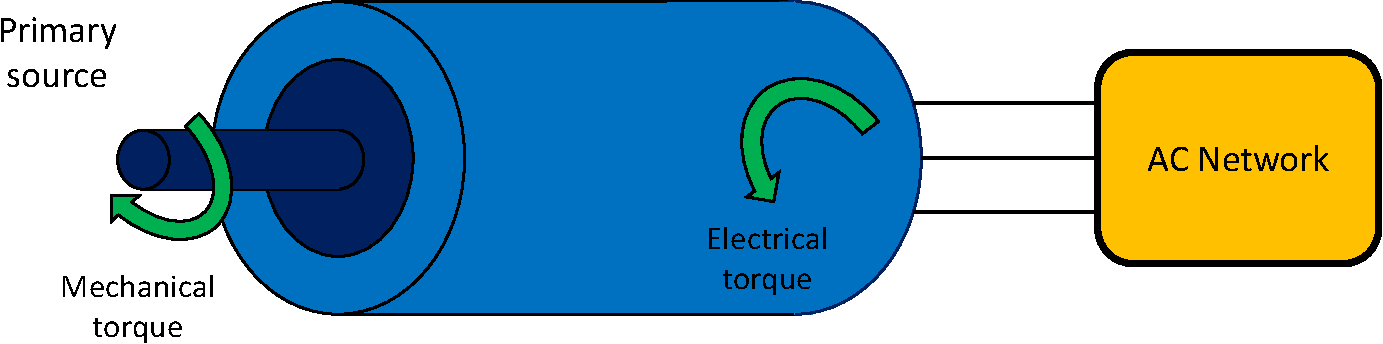
\includegraphics[height = 3cm,width = 12.5cm]{Diagrams/Chapter_1/Energy_conv_system.pdf}
    \caption{Conventional generators connection to the AC network \cite{denis_migrate_2018}}
    \label{fig:Energy_conv_system}
\end{figure}

%\section*{Small scale offshore networks}
The majorly contributing source among the available \gls{RES} is wind energy. Specifically, offshore wind energy is predicted to be the most significant source of energy among the North Sea countries by 2040 \cite{muller2017translate}. As a result, the deployment of offshore wind energy technology is expected to grow further. With the increase in integration of offshore wind energy, the inherent characteristics of offshore wind energy conversion systems will affect the nature of the power system. The vulnerable wind speed conditions due to the uncertain behaviour of wind, could lead to variations in the supply and demand and therefore, fluctuations in voltages and frequency are bound to occur. Moreover, as the power systems become weak due to the decommissioning of synchronous generators in conventional power plants that use non-renewable sources, the integration of offshore wind power plants to such weak power systems pose various research challenges on the power system stability. 


One among the challenge is related to voltage stability. The continuous variations in offshore wind speed causes constant change in the active power output of the offshore wind power plant. This could lead to an increase in the reactive power output and consequently voltage at the point of common coupling (\gls{PCC}). The conventional current control methods using Proportional Integral (\gls{PI}) controllers in the modern Wind Generators (\gls{WG}s) are capable of providing voltage control by injecting reactive currents when connected to a strong network \footnote{SCR = SC$_{MVA}$/P;\; where SC$_{MVA}$ is the short circuit power of the network and P is the active power generation. \\
If SCR = 100 to 250, it is a strong grid. If SCR = 5 to 25, it is a weak grid.}. However, these controllers are not suitable for operation in highly \gls{PE} converter dominated grids as the connected network is weak and is not capable of absorbing the injected currents. Furthermore, during the scenario of islanding, voltage control by the conventional current controllers is ineffective as the deviation in voltage is not high enough to activate a productive voltage reduction mechanism. There are challenges in terms of frequency stability  as well since the conventional current controllers in the \gls{WG}s are not equipped to provide frequency control of the network during islanding. 

Currently, the state-of-the-art technology for the transfer of offshore wind power to the onshore system is Voltage Source Converter (\gls{VSC}) based  - High Voltage Direct Current (\gls{HVDC}) transmission links. Presently, Modular Multi-level Converter (\gls{MMC}) topology that falls under the classification of \gls{VSC} topologies is the most suitable solution. Few of the advantages of \gls{MMC} are \cite{cigre_B455}, (1) ease of integration with Offshore Wind Farms (\gls{OWF})s, (2) supporting bi-directional flow of power between the offshore network and onshore system, and (3) independent control of active and reactive powers in the network. However, with the available technology, \gls{MMC}-\gls{HVDC} transmission are limited to a rated capacity of 1.2 GW \cite{peralta2012detailed}.

%\section*{Large scale offshore networks}\label{large_scale_intro}
The implementation of large scale offshore networks (greater than or equal to 2 GW) creates a highly \gls{PE} converter dominated network. The aforementioned challenges in terms of voltage and frequency control by the \gls{PE} converters without the presence of conventional units is prominent in large scale offshore networks. 

The absence of conventional generators would mean that the \gls{PE} converters will have to take into account the decreasing inertia of the system that leads to a faster dynamic behaviour and needs controllers with faster time response. Moreover, in large scale offshore networks, distant \gls{OWF}s would be connected in parallel. With parallel operation of the conventional current controllers in \gls{WG}s, interactions can persist among them and could lead to instability of the network. Additionally, the restoration of grid following disturbances by the \gls{PE} converter units is a serious matter of concern. With the conventional current control approach, grid restoration is challenging without the help of auxiliary diesel generators. However, in the case of large scale offshore networks, the role of grid restoration must be taken up by \gls{PE} converters. There can be arguments that storage facilities such as battery and thermal can be a realizable solution in case when there are no conventional generators available. Huge investment costs, low lifetime and low efficiency when compared to controller modifications are the drawbacks that make these storage facilities practically unusable in large scale offshore networks \cite{telaretti_economic_2016}.

Traditionally, the transmission of power from \gls{OWF} to the offshore converter station uses a combination of 33 kV and 145 kV \gls{HVAC} cables. The \gls{OWF}s are connected to an \gls{AC} offshore platform using 33 kV \gls{HVAC} cables. The platform holds a power transformer that is used to step-up voltage from 33 kV to 145 kV, and power is transferred from the \gls{AC} platform to the offshore converter station using 145 kV \gls{HVAC} cables \cite{abdelwahed2016power}. However, the upcoming projects are expected to have a higher voltage level of 66 kV for transmission to allow twice the amount of power transferred compared to 33 kV. Therefore, this would only require 66 kV \gls{HVAC} cables to directly connect \gls{OWF}s to offshore converter station, avoiding the use of an \gls{AC} collector platform \cite{dnv66kv}. Hence, advancing towards large scale offshore networks, it would be more appropriate to assess the performance of these networks developed with 66 kV \gls{HVAC} transmission. 

% On the \gls{OWF} side, conventionally, the \gls{OWF}s are connected to a \gls{AC} collector platform through 33 kV cables. At the platform, a 33/145 kV transformer is used to step-up the voltage and the power is transferred to the offshore converter station using 145 kV cables. However, the upcoming projects plan to have a rating of 66 kV \gls{HVAC} transmission compared to the conventional combination of 33 kV and 145 kV \gls{HVAC} transmission due to the advantages of lesser array cabling and higher power transmission. In such cases, the \gls{AC} collector platform can be avoided and power can transmitted from the \gls{OWF}s to the offshore converter station directly using 66 kV \gls{HVAC} cables \cite{dnv66kv}.

With the available \gls{MMC}-\gls{HVDC} transmission technology, multiple \gls{MMC}-\gls{HVDC} transmission links connected in parallel would be required to transfer the bulk amount of offshore wind power generated from large scale offshore networks to the onshore system. In such networks, the power flow between the parallel operated \gls{MMC}s and the \gls{OWF}s must be coordinated during steady state and dynamic conditions. The major challenges regarding voltage and frequency control during islanding of the \gls{OWF}s must be taken into account. The scenario of reactive current injection that needs to be provided by the \gls{WG}s during dynamic conditions as demanded by majority of the grid codes must also be taken into consideration \cite{mohseni_review_2012}. Therefore, the progress towards the development of large scale offshore networks calls for a generic model with a suitable layout with the available technology that is capable of tackling the aforementioned technical challenges and providing stable operation during steady state and dynamic conditions. 
% the connection of distant \gls{OWF}s also creates challenges for the system operators. High Voltage Direct Current (\gls{HVDC}) transmission is preferred over High Voltage Alternating Current (\gls{HVAC}) for longer distances due to lower losses and lower investment costs \cite{ryndzionek_evolution_2020}. Conventionally, 


\section{Literature Review}

As seen in Section \ref{Background}, the major challenges are; development of large scale offshore networks with available technology is challenging, no much knowledge about 66 kV \gls{HVAC} transmission available, and new control strategies are required that can provide better control of voltage and frequency. Hence, a generic model for large scale offshore networks with the latest trend in available technology, and enhanced control strategies is a key research requirement. 
% The literature review is mainly focused on three aspects: 1) control strategies to overcome the technical challenges related to voltage and frequency control in \gls{WG}s, 2) power transfer from the \gls{OWF}s to the offshore \gls{MMC} converter and 3) topology of  
% Going with the latest trend, different approaches are available for connection of \gls{MMC}s.

Based on \gls{MMC}-\gls{HVDC} transmission technology, there are mainly three configurations available for the connection of offshore and onshore converter stations \cite{cigre_B455}, \cite{sharifabadi2016design}: 
\begin{itemize}
    \item Point-to-point connection: The configuration connects one \gls{OWF} to the offshore converter station, which is then connected using \gls{HVDC} link to the onshore converter station.
    \item Multi-infeed connection: The configuration involves connecting one \gls{OWF} to two different onshore systems by connecting two offshore converter stations on a common bus on the Alternating Current (\gls{AC}) side and transmitting power through two \gls{HVDC} links. Such a configuration allows for increasing the rating of the \gls{OWF} beyond the capacity of a single offshore converter station. The drawback of such a configuration is that, it allows the connection of only one \gls{OWF} to the network.
    \item Multi-Terminal Direct
    Current (MTDC) connection: In this configuration, the \gls{HVDC} links of multiple offshore converter stations are connected to a main Direct Current (\gls{DC}) link. Such a configuration enables transfer of active power to the onshore system depending on the capacity of the main \gls{DC} link. The drawback of such a configuration is that, a complete shut down and restart of the connected \gls{MMC}s is required for a fault on the \gls{DC} side.
\end{itemize}

The multi-infeed and the MTDC connections allow for parallel operation of \gls{MMC}s which is a significant requirement for large scale offshore networks with the available technology. But both the configurations have the drawback of being able to connect only one \gls{OWF} to the network. Therefore, configurations that utilize several \gls{OWF}s with parallel operation of \gls{MMC}s are currently unavailable and is a key area of research. The topology mentioned in \cite{lozada_ayala_dynamic_2018} embraces the utilization of 66 kV \gls{HVAC} transmission from the \gls{OWF}s (all connected in parallel) to the offshore converter station. However, the topology examined does not utilize parallel operation of \gls{MMC}s and uses only one \gls{MMC}-\gls{HVDC} link with a maximum power transfer capacity of 1 GW.

% On the \gls{OWF} side, 

%The technical challenges regarding voltage and frequency control are key aspects to be considered for the development of large scale networks.
Typically, \gls{PE} converters in the \gls{WG}s are connected to the network for parallel operation using present state-of-the-art technology, current control strategies. In such control strategies, the regulation of power output of the converters is achieved by measuring the angle of the grid voltage. The drawback of these control strategies is that they require an already existing reference voltage. There are control strategies that create the reference voltage and are termed as voltage control strategies. One among the voltage control strategies is the V/F (voltage/frequency) control that is utilized for operation in the islanded mode. The drawback with V/F control is that it is not equipped for the parallel operation of various voltage forming converter units \cite{weise2019comparison}. Therefore, there needs to be new control strategies in the \gls{WG}s that can create the reference voltage and work in parallel operation. Such control strategies are an emerging area of research. There are studies performed to implement control strategies that can create voltage reference and work in parallel operation as well. Few among them are mentioned as follows:

% European Network of Transmission System Operators for Electricity (ENTSO-E) classifies converters into three classes (Class 1, Class 2 and Class 3) and the converters working with the strategies mentioned above are categorized under Class 3. The complete requirements that need to be complied by such converters are depicted in \cite{christensen2020high}.

\begin{itemize}
    \item Virtual Synchronous Machines (VSM): The \gls{PE} converter control is modelled with the characteristics of a synchronous machine in terms of inertia and voltage support by correspondingly deriving the equations \cite{markovic2018lqr}, \cite{duckwitz_operating_behavior}, \cite{lu_virtual_2019}.
    
    \item Modified Droop Control:
    This strategy is common for standalone grids, where the parallel operation of voltage forming units is developed recently using the f/P (frequency/active power) and V/Q (voltage/reactive power) droop controls similar to the control in synchronous generators \cite{bouzid2016simulation}. Few authors have named these droop control concepts as Virtual Synchronous Machines Without Inertia (VSCM0H) \cite{yu2016use}.
    
    \item Direct Voltage Control (\gls{DVC}):
    \gls{DVC} is a representation of the conventional current control approach towards a voltage control. \gls{DVC} allows for the direct control of the \gls{AC} converter voltage which in turn varies the current injected by the converter  \cite{korai_dynamic_2019}, \cite{erlich_new_2017}. This approach provides continuous voltage control both in steady-state and dynamic scenarios. %This control method is implemented for analysis in this thesis work.
    
    \item Extended Current Control:
    The control is similar to the conventional current control with an additional inertia control in the outer control loop by using a synthetic inertia controller that gives a behaviour similar to that of a synchronous machine \cite{duckwitz_derivation_2019} \cite{liu2017control}. 
\end{itemize}

Studies of I. Erlich et al. and A. Korai et al. in \cite{erlich_new_2017} and \cite{korai_dynamic_2019} show appealing results of the implemented \gls{DVC} for highly \gls{PE} dominated systems. The simulations are tested for different grids based on real world data and provide promising outcomes with effective voltage and frequency control. Hence, with such proven results and available models, the \gls{DVC} strategy was chosen to be incorporated for this work. Moreover, the real-time implementation of \gls{DVC} in Type-4 \gls{WG} is attempted in \cite{sethi_real-time_nodate-new}, but the latest trend of 66 kV \gls{HVAC} transmission and the major requirement of reactive current injection by the \gls{WG}s during dynamic conditions is lacking.

It is also good to analyze the effectiveness of other control strategies mentioned above. With a generic offshore network model, different control strategies can be implemented in the \gls{OWF}s and the complexity related to the interoperability of the controllers can be assessed. However, this lies beyond the scope of this project.

\section{Objectives and Research Questions}
The overall goal of the thesis is to develop a generic digital twin model of 2 GW, 66 kV \gls{HVAC} offshore network and to perform analysis on the dynamics of voltage and power at various locations in the network. The thesis makes use of the Electro-Magnetic Transient (\gls{EMT}) simulation-based software tools such as RSCAD and PowerFactory to analyze the performance of the developed control models. The average model of Type-4 \gls{WG} available in RSCAD is used as a starting point. The thesis provides a detailed description of the different available features in RSCAD that are employed to develop the 2 GW model. 
To achieve the overall goal, the following research questions are defined:
\begin{itemize}
    \item How effective is the Direct Voltage Control (\gls{DVC}) when implemented in an \gls{EMT} average model of Type-4 \gls{WG} connected to a 66 kV equivalent \gls{HVAC} system in RSCAD?
    
    \item What insights can be attained by the \gls{EMT} average model of Type-4 \gls{WG} with \gls{DVC} in 66 kV network in RSCAD in comparison with a similar network modelled with a simplified Type-4 \gls{WG} configuration with \gls{DVC} in DIgSILENT PowerFactory?
    
    \item How can Type-4 \gls{WG}s with implemented \gls{DVC} work in coordination with offshore \gls{MMC}s within a multi-gigawatt offshore transmission network?
    
    \item How effectively do Type-4 \gls{WG}s with implemented \gls{DVC} perform when connected in an offshore network for parallel operation?

\end{itemize}

\section{Thesis Contribution}
On behalf of the thesis objectives defined above, the key contributions from this thesis are presented in this section.

\begin{itemize}
    \item Implementation of the \gls{DVC} in Type-4 \gls{WG} model in RSCAD for an offshore 66 kV \gls{HVAC} network. With proper documentation provided in this report, the developed 66 kV \gls{HVAC} model in RSCAD can be utilized for future work.
    
    \item Development of a 66 kV \gls{HVAC} offshore network in PowerFactory by adapting the benchmark \gls{DVC} model in Type-4 \gls{WG}s. With proper documentation provided in this report, the developed 66 kV \gls{HVAC} model in PowerFactory model can be utilized for future work.
    
    \item Development of a digital twin of 2 GW, 66 kV \gls{HVAC} offshore network with \gls{DVC} implemented in Type-4 \gls{WG}s connected to two offshore converter stations in RSCAD. With proper documentation provided in this report, the developed 2 GW model in RSCAD can be utilized for future work.
    
    \item Automation script for the operation of the developed 2 GW offshore network model using the interface between RSCAD and MATLAB is created. %With proper documentation provided in this report, the script can be utilized for future work.
\end{itemize}

\section{Thesis Outline}
A brief outline of the methodology is structured in several chapters, which sequentially describe the performed tasks as follows:
\begin{itemize}
    \item Chapter \ref{2}: The chapter presents the concepts of wind energy conversion system and the classification of wind turbines. The overview of the \gls{OWF} network with all the major equipment and the latest trend in technology is explained. The issues with the present current control strategies and the necessity to move towards better control strategies are addressed. The new control strategy, \gls{DVC}, to be implemented in Type-4 \gls{WG} is formulated.  
    
    \item Chapter \ref{3}: The implementation of \gls{DVC} in \cite{korai_dynamic_2019} and \cite{sethi_real-time_nodate-new} for a digital twin of 66 kV \gls{HVAC} offshore network in RSCAD is detailed. The performance of Type-4 \gls{WG} with \gls{DVC}, in terms of short-term voltage stability and reactive current injection, under severe disturbances is analyzed. Modelling of a similar 66 kV \gls{HVAC} offshore network in DIgSILENT PowerFactory tool is also addressed. The comparison of the dynamic performance of \gls{DVC} in two \gls{EMT} platforms (RSCAD and PowerFactory) for a 66 kV \gls{HVAC} offshore network during severe disturbances is carried out. 
    
    \item Chapter \ref{4}: The development of a large scale digital twin model of a 2 GW offshore network in RSCAD is detailed. The modifications in the control structures of the \gls{MMC}s to work in coordination with the implemented \gls{DVC} in \gls{WG}s are addressed.
    
    \item Chapter \ref{5}: The operation of the developed large scale 2 GW network is discussed. The interplay of offshore \gls{MMC}s and Type-4 \gls{WG}s in terms of dynamic power flow control within the offshore network (by analyzing the voltage and current profiles in the electrical path between the \gls{WG}s and the \gls{MMC}s) is performed. 
    
    \item Chapter \ref{6}: The significant conclusions for the research questions are provided. The future scope and recommendations are also added.
\end{itemize}

A figurative representation of the thesis workflow is presented in Figure \ref{fig:Thesis_outline}.

\begin{figure}[H]
\centering
%\hspace*{-1.2cm}
    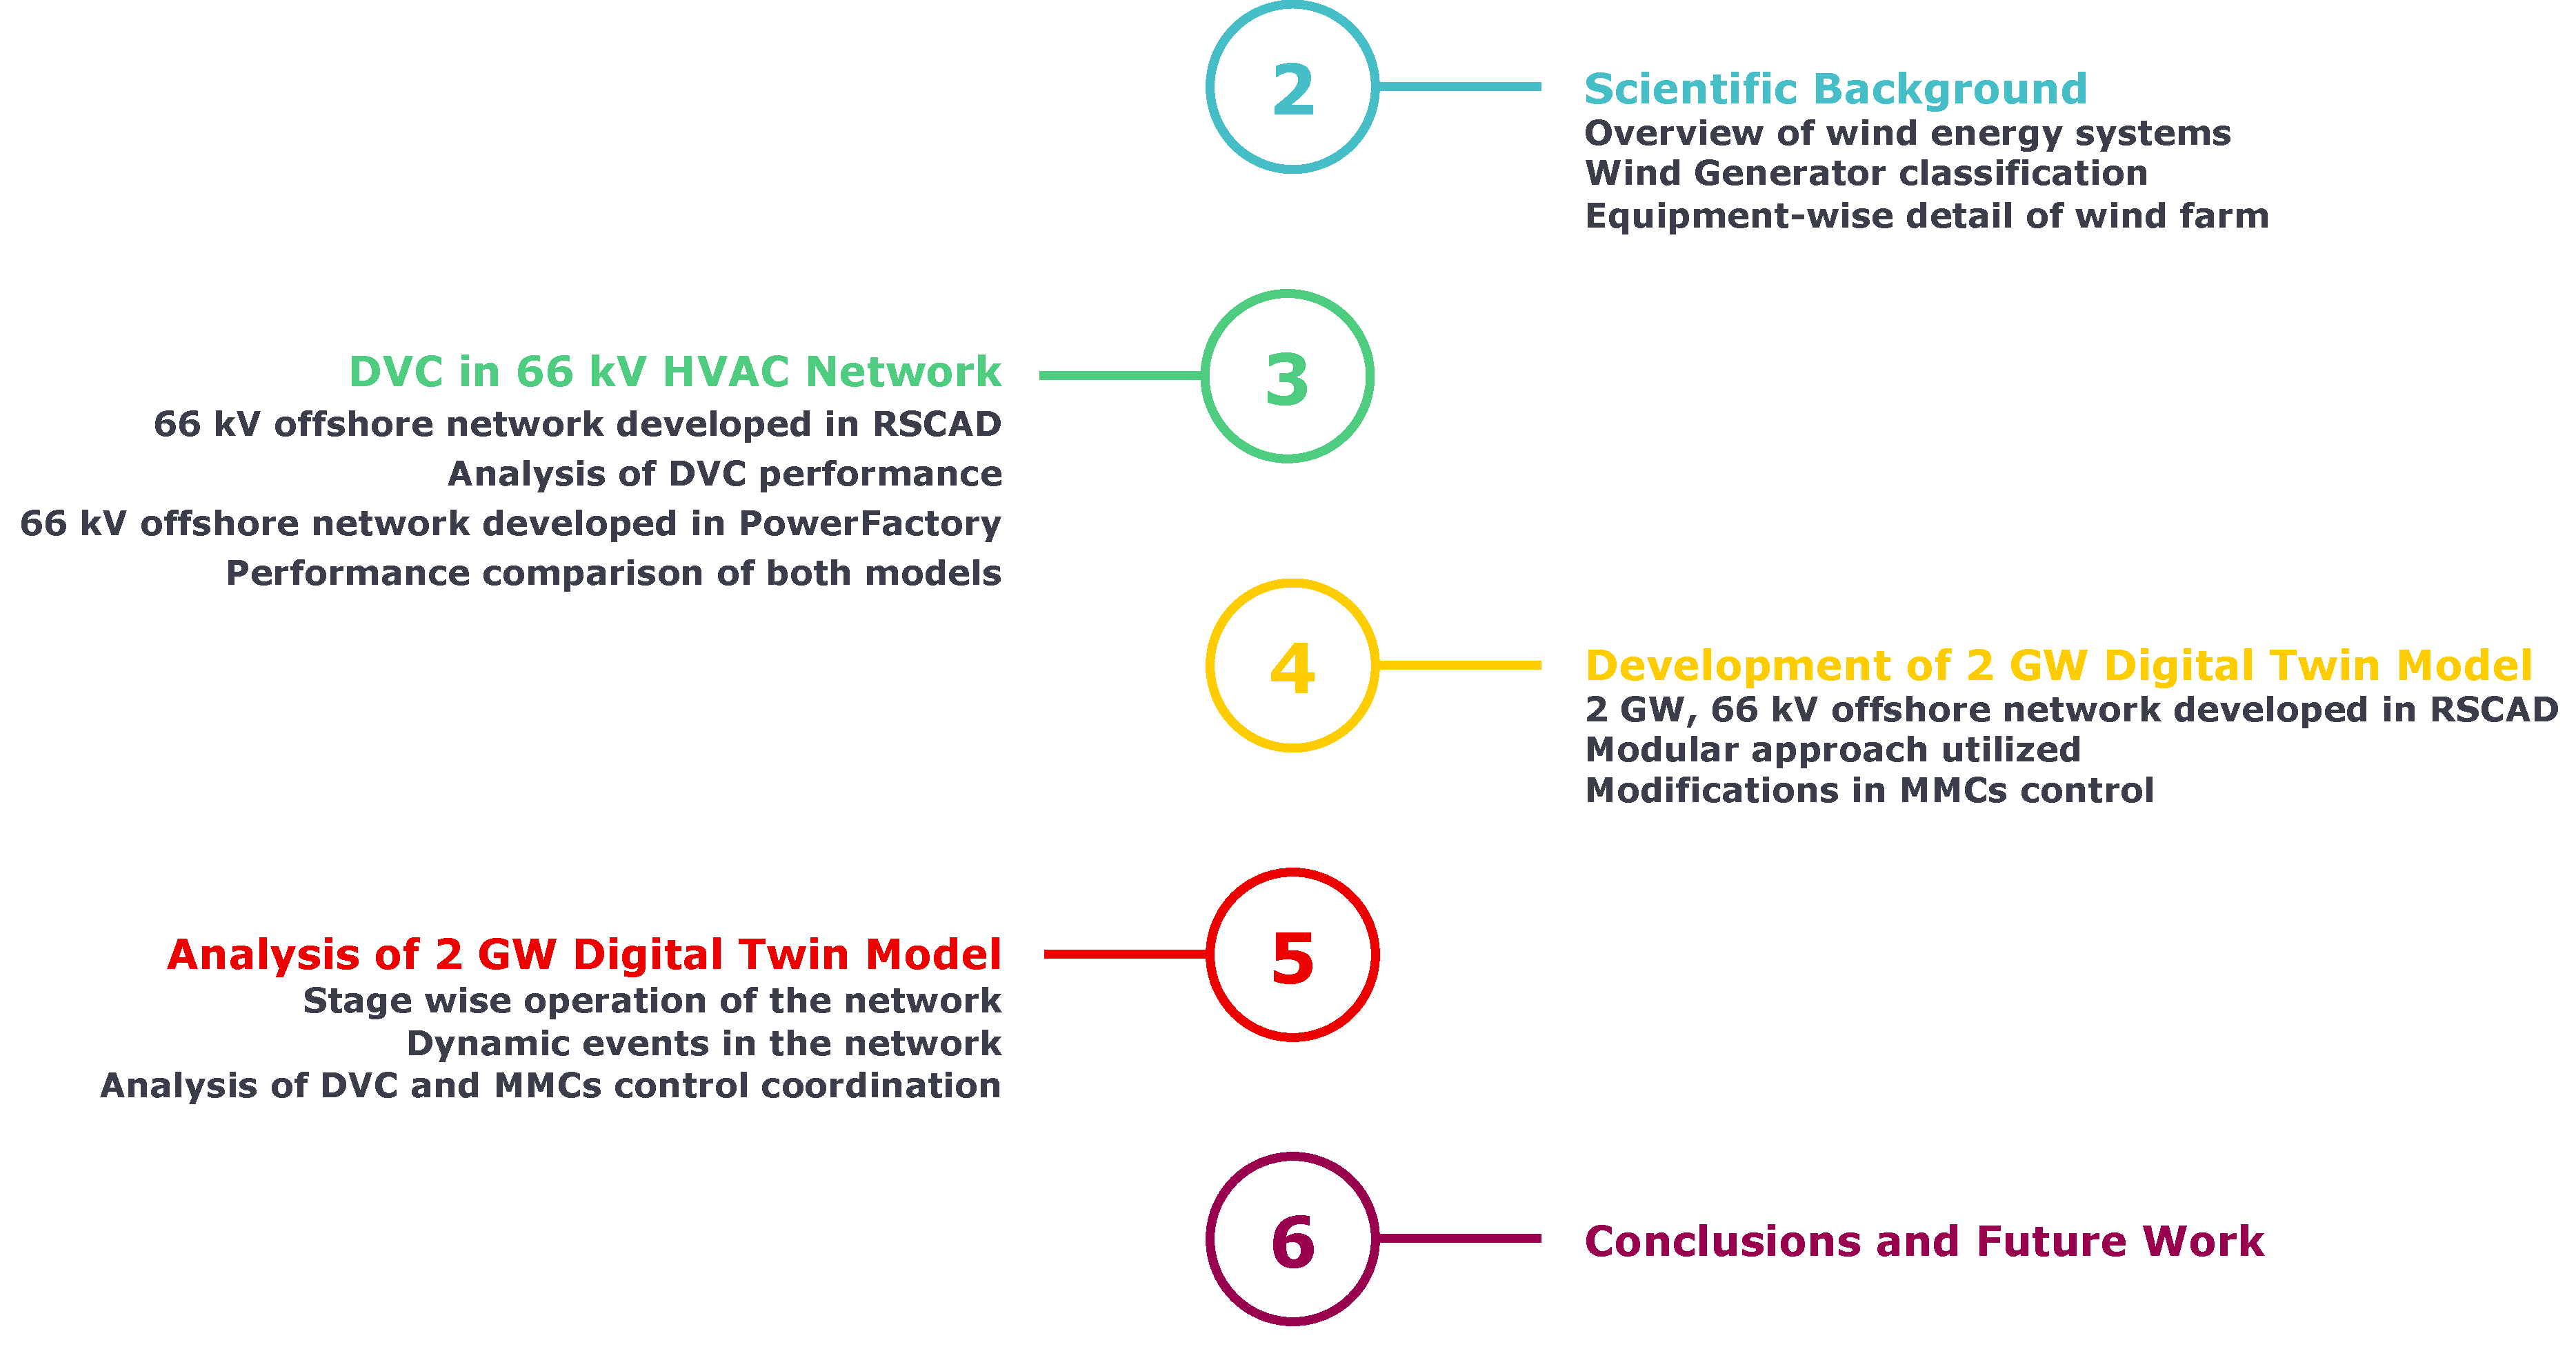
\includegraphics[height = 9.5cm,width =\textwidth]{Diagrams/Chapter_1/Thesis_flowchart.pdf}
    \caption{Work flow of thesis}
    \label{fig:Thesis_outline}
\end{figure}
